%======================================================================
% AI-Powered Knowledge Work – Modern Professional Presentation
%======================================================================
\documentclass[aspectratio=169,14pt]{beamer}

%---------------------------------------------------------------------
% Modern Theme & Packages
%---------------------------------------------------------------------
\usetheme{Boadilla}
\usecolortheme{whale}
\usefonttheme{professionalfonts}

\usepackage[utf8]{inputenc}
\usepackage{graphicx}
\usepackage{booktabs}
\usepackage{tikz}
\usepackage{fontawesome5}
\usepackage{hyperref}
\usepackage{multicol}
\usepackage{xcolor}
\usepackage{tcolorbox}
\usepackage{pgfplots}
\pgfplotsset{compat=1.18}
\usepackage{soul}
\usepackage{ragged2e}
\usepackage{etoolbox}
\usepackage{microtype}

% Modern fonts
\usepackage[sfdefault]{FiraSans}
\usepackage{FiraMono}
\usepackage[mathrm=sym]{unicode-math}

%---------------------------------------------------------------------
% Professional Color Palette
%---------------------------------------------------------------------
\definecolor{primaryblue}{RGB}{0,123,255}
\definecolor{deepblue}{RGB}{0,90,200}
\definecolor{accentcyan}{RGB}{0,188,212}
\definecolor{successgreen}{RGB}{76,175,80}
\definecolor{warningorange}{RGB}{255,152,0}
\definecolor{modernpurple}{RGB}{103,58,183}
\definecolor{elegantgray}{RGB}{96,125,139}
\definecolor{lightbg}{RGB}{248,249,250}
\definecolor{darktext}{RGB}{33,37,41}
\definecolor{pgffillcolor}{RGB}{0,188,212}

%---------------------------------------------------------------------
% Modern Beamer Configuration
%---------------------------------------------------------------------
\setbeamertemplate{navigation symbols}{}
\setbeamertemplate{footline}[frame number]
\setbeamercolor{normal text}{fg=darktext}
\setbeamercolor{structure}{fg=deepblue}
\setbeamercolor{frametitle}{fg=white,bg=deepblue}
\setbeamercolor{title}{fg=white}
\setbeamercolor{subtitle}{fg=accentcyan}
\setbeamercolor{block title}{fg=white,bg=primaryblue}
\setbeamercolor{block body}{fg=darktext,bg=lightbg}

% Modern frame title
\setbeamertemplate{frametitle}{%
  \nointerlineskip
  \begin{beamercolorbox}[wd=\paperwidth,sep=0pt,leftskip=20pt,rightskip=20pt]{frametitle}
    \vspace{15pt}
    {\Large\bfseries\insertframetitle}
    \vspace{15pt}
  \end{beamercolorbox}
}

% Rounded blocks
\tcbuselibrary{skins,breakable}
\newtcolorbox{modernblock}[2][]{%
  colback=lightbg,
  colframe=#2,
  fonttitle=\bfseries,
  coltitle=white,
  colbacktitle=#2,
  boxrule=0pt,
  arc=4mm,
  left=10pt,right=10pt,top=10pt,bottom=10pt,
  title=#1
}

%---------------------------------------------------------------------
% Advanced Background System
%---------------------------------------------------------------------
\newcommand{\ModernBackground}[1]{%
  \setbeamertemplate{background}{%
    \begin{tikzpicture}[remember picture,overlay]
      % Gradient overlay
      \fill[white,opacity=0.95] (current page.south west) rectangle (current page.north east);
      \shade[left color=primaryblue!10,right color=accentcyan!5,opacity=0.3]
        (current page.south west) rectangle (current page.north east);
      % Image with artistic overlay
      \node[anchor=center,opacity=0.15] at (current page.center) {
        \includegraphics[width=\paperwidth,height=\paperheight,keepaspectratio]{#1}
      };
      % Modern geometric elements
      \fill[primaryblue,opacity=0.05] ([xshift=-100pt,yshift=-50pt]current page.north east)
        circle (200pt);
      \fill[accentcyan,opacity=0.05] ([xshift=100pt,yshift=50pt]current page.south west)
        circle (150pt);
    \end{tikzpicture}}
}

% Clean background for content slides
\newcommand{\ContentBackground}{%
  \setbeamertemplate{background}{%
    \begin{tikzpicture}[remember picture,overlay]
      \fill[white] (current page.south west) rectangle (current page.north east);
      \shade[top color=lightbg,bottom color=white,opacity=0.5]
        (current page.south west) rectangle (current page.north east);
    \end{tikzpicture}}
}

%---------------------------------------------------------------------
% Custom Commands
%---------------------------------------------------------------------
\newcommand{\highlight}[1]{\textcolor{primaryblue}{\textbf{#1}}}
\newcommand{\stat}[2]{{\Huge\textbf{#1}}\\{\small #2}}
\newcommand{\impactitem}[2]{\item[\textcolor{#1}{\faCheckCircle}] #2}

%---------------------------------------------------------------------
% Document Metadata
%---------------------------------------------------------------------
\title{\Huge\textbf{AI-Powered Knowledge Work}}
\subtitle{\Large Master the New Universal Workspace}
\author{\textbf{Dr. John O'Hare}}
\institute{DREAMLAB | Chief Hallucination Officer}
\date{2025 Workshop Series}

%=====================================================================
% Document Body
%=====================================================================
\begin{document}

% Title Slide with Modern Design
\ModernBackground{slide-1-backdrop.png}
\begin{frame}[plain]
  \begin{tikzpicture}[remember picture,overlay]
    % Dark overlay for text contrast
    \fill[deepblue,opacity=0.9] (current page.south west) rectangle (current page.north east);
    % Geometric accent
    \fill[accentcyan,opacity=0.3] ([xshift=-100pt]current page.east)
      -- ([yshift=100pt]current page.south east)
      -- (current page.south east)
      -- cycle;
  \end{tikzpicture}
  \centering
  \vspace{2cm}
  {\color{white}\Huge\textbf{AI-Powered Knowledge Work}}\\[0.5cm]
  {\color{accentcyan}\Large Transform Your Professional Practice in 5 Days}\\[1cm]
  {\color{white}\large\textbf{Dr. John O'Hare}}\\[0.2cm]
  {\color{white!80}\small DREAMLAB | Chief Hallucination Officer}\\[1cm]
  {\color{accentcyan}\faCalendar\quad March 17-21, 2025}
\end{frame}

% The Revolution Slide
\ContentBackground
\begin{frame}[t]
  \frametitle{The AI Revolution Has Two Classes}

  \begin{columns}[T]
    \column{0.48\textwidth}
    \begin{modernblock}[The 95\%]{warningorange}
      \begin{itemize}
        \item Copy-paste from ChatGPT
        \item \$20/month for limitations
        \item No version control
        \item Manual repetitive tasks
        \item Consumer-grade results
      \end{itemize}
    \end{modernblock}

    \column{0.48\textwidth}
    \begin{modernblock}[The 5\%]{successgreen}
      \begin{itemize}
        \item Direct API access
        \item Pay pennies per task
        \item Full automation control
        \item 10× productivity gains
        \item Professional-grade output
      \end{itemize}
    \end{modernblock}
  \end{columns}

  \vspace{0.5cm}
  \centering
  \begin{tcolorbox}[colback=primaryblue!10,colframe=primaryblue,boxrule=2pt,arc=3mm,width=0.8\textwidth]
    \centering\large\textbf{Which side will you choose?}
  \end{tcolorbox}
\end{frame}

% Transformation Stats
\ModernBackground{slide-3-backdrop.png}
\begin{frame}[t]
  \frametitle{Real Impact, Real Numbers}

  \begin{columns}[T]
    \column{0.25\textwidth}
    \centering
    \begin{tcolorbox}[colback=primaryblue!20,colframe=primaryblue,arc=3mm,boxrule=0pt]
      \centering
      \stat{70\%}{Time saved on\\grant writing}
    \end{tcolorbox}

    \column{0.25\textwidth}
    \centering
    \begin{tcolorbox}[colback=successgreen!20,colframe=successgreen,arc=3mm,boxrule=0pt]
      \centering
      \stat{5×}{Faster business\\documentation}
    \end{tcolorbox}

    \column{0.25\textwidth}
    \centering
    \begin{tcolorbox}[colback=warningorange!20,colframe=warningorange,arc=3mm,boxrule=0pt]
      \centering
      \stat{10×}{Research\\throughput}
    \end{tcolorbox}

    \column{0.25\textwidth}
    \centering
    \begin{tcolorbox}[colback=modernpurple!20,colframe=modernpurple,arc=3mm,boxrule=0pt]
      \centering
      \stat{£2M}{Funding won\\by alumni}
    \end{tcolorbox}
  \end{columns}

  \vspace{0.8cm}
  \begin{center}
    \large\textit{"The gap between AI users and AI masters is widening daily."}
  \end{center}
\end{frame}

% Who Is This For - Visual
\ContentBackground
\begin{frame}[t]
  \frametitle{Perfect For Knowledge Workers}

  \begin{columns}[T]
    \column{0.33\textwidth}
    \centering
    \textcolor{primaryblue}{\Huge\faUserGraduate}\\[0.3cm]
    \textbf{Academics}\\
    \small Grant proposals\\Research papers\\Literature reviews

    \column{0.33\textwidth}
    \centering
    \textcolor{successgreen}{\Huge\faChartLine}\\[0.3cm]
    \textbf{Business Leaders}\\
    \small Strategic documents\\Reports \& analysis\\Knowledge systems

    \column{0.33\textwidth}
    \centering
    \textcolor{warningorange}{\Huge\faLightbulb}\\[0.3cm]
    \textbf{Consultants}\\
    \small Client deliverables\\Rapid prototyping\\Project automation
  \end{columns}

  \vspace{0.8cm}
  \begin{tcolorbox}[colback=lightbg,colframe=elegantgray,boxrule=1pt,arc=3mm]
    \centering
    \large\textbf{No coding required} – If you can use Word, you're ready
  \end{tcolorbox}
\end{frame}

% Journey Overview - Modern Visual
\ModernBackground{slide-5-backdrop.png}
\begin{frame}[t]
  \frametitle{Your 5-Day Transformation Journey}

  \begin{tikzpicture}[remember picture,overlay]
    % Timeline
    \draw[line width=3pt,primaryblue] ([xshift=2cm,yshift=-1cm]current page.north west) -- ([xshift=-2cm,yshift=-1cm]current page.north east);

    % Day markers
    \foreach \x/\day/\title/\color in {
      0.2/1/Universal Workspace/primaryblue,
      0.35/2/AI Partners/successgreen,
      0.5/3/Private Brain/warningorange,
      0.65/4/AI Teams/modernpurple,
      0.8/5/Publishing/accentcyan
    }{
      \node[circle,fill=\color,text=white,minimum size=1cm,font=\bfseries] at ([xshift=\x*\paperwidth-0.5\paperwidth,yshift=-1cm]current page.north) {\day};
      \node[below,text width=2.5cm,align=center,font=\small] at ([xshift=\x*\paperwidth-0.5\paperwidth,yshift=-2cm]current page.north) {\title};
    }
  \end{tikzpicture}

  \vspace{3cm}
  \begin{columns}[T]
    \column{0.5\textwidth}
    \textbf{Start:} AI Consumer\\
    \small Limited to web interfaces

    \column{0.5\textwidth}
    \raggedleft
    \textbf{Finish:} AI Commander\\
    \small Complete automation mastery
  \end{columns}
\end{frame}

% Day 1 - Modern Layout
\ContentBackground
\begin{frame}[t]
  \frametitle{Day 1: Your AI Command Center}

  \begin{columns}[T]
    \column{0.5\textwidth}
    \begin{modernblock}[Morning Session]{primaryblue}
      \textbf{VS Code Transformation}
      \begin{itemize}
        \item AI-powered extensions
        \item Container environments
        \item Professional workspace
        \item Version control mastery
      \end{itemize}
    \end{modernblock}

    \column{0.5\textwidth}
    \begin{modernblock}[Afternoon Session]{accentcyan}
      \textbf{Visual Project Management}
      \begin{itemize}
        \item Mermaid diagrams
        \item Gantt charts
        \item Process flows
        \item Knowledge maps
      \end{itemize}
    \end{modernblock}
  \end{columns}

  \vspace{0.5cm}
  \centering
  \begin{tcolorbox}[colback=successgreen!20,colframe=successgreen,boxrule=2pt,arc=3mm,width=0.9\textwidth]
    \centering
    \faCheckCircle\quad\textbf{Day 1 Achievement:} Professional AI workspace with visual project plan
  \end{tcolorbox}
\end{frame}

% Day 2 - Vibe Coding
\ModernBackground{slide-9-backdrop.png}
\begin{frame}[t]
  \frametitle{Day 2: "Vibe Coding" Revolution}

  \begin{center}
    \Large\textbf{Describe what you want → AI builds it perfectly}
  \end{center}

  \vspace{0.5cm}

  \begin{columns}[T]
    \column{0.33\textwidth}
    \centering
    \textcolor{primaryblue}{\Huge\faComments}\\[0.3cm]
    \textbf{Natural Language}\\
    \small Just describe your vision

    \column{0.33\textwidth}
    \centering
    \textcolor{successgreen}{\Huge\faCode}\\[0.3cm]
    \textbf{AI Creates}\\
    \small Complete implementations

    \column{0.33\textwidth}
    \centering
    \textcolor{warningorange}{\Huge\faGlobe}\\[0.3cm]
    \textbf{Deploy Live}\\
    \small Online in minutes
  \end{columns}

  \vspace{0.8cm}
  \begin{modernblock}[Live Demo Examples]{deepblue}
    \centering
    Business website • Interactive dashboard • Documentation site • Portfolio
  \end{modernblock}
\end{frame}

% Day 3 - Private AI
\ContentBackground
\begin{frame}[t]
  \frametitle{Day 3: Your Private AI Brain}

  \begin{tikzpicture}[remember picture,overlay]
    % Security badge
    \node[anchor=north east] at ([xshift=-20pt,yshift=-80pt]current page.north east) {
      \textcolor{successgreen}{\Huge\faShieldAlt}
    };
  \end{tikzpicture}

  \begin{columns}[T]
    \column{0.5\textwidth}
    \begin{modernblock}[100\% Private]{successgreen}
      \begin{itemize}
        \item Runs on YOUR laptop
        \item No internet required
        \item Complete data privacy
        \item Zero subscription fees
      \end{itemize}
    \end{modernblock}

    \column{0.5\textwidth}
    \begin{modernblock}[RAG System]{modernpurple}
      \begin{itemize}
        \item Reads all your documents
        \item Instant answers
        \item Exact citations
        \item Your knowledge on tap
      \end{itemize}
    \end{modernblock}
  \end{columns}

  \vspace{0.5cm}
  \centering
  \textit{"What did we decide in the March meeting?"} → \highlight{Instant answer with source}
\end{frame}

% Day 4 - AI Teams Visual
\ModernBackground{slide-11-backdrop.png}
\begin{frame}[t]
  \frametitle{Day 4: Deploy Your AI Workforce}

  \begin{center}
    \begin{tikzpicture}
      % Central node
      \node[circle,fill=primaryblue,text=white,minimum size=2cm] (center) at (0,0) {\textbf{You}};

      % Agent nodes
      \node[circle,fill=successgreen,text=white,minimum size=1.5cm] (research) at (-3,2) {\faSearch};
      \node[circle,fill=warningorange,text=white,minimum size=1.5cm] (writer) at (3,2) {\faPen};
      \node[circle,fill=modernpurple,text=white,minimum size=1.5cm] (analyst) at (-3,-2) {\faChartBar};
      \node[circle,fill=accentcyan,text=white,minimum size=1.5cm] (auto) at (3,-2) {\faRobot};

      % Connections
      \draw[thick,->] (center) -- (research);
      \draw[thick,->] (center) -- (writer);
      \draw[thick,->] (center) -- (analyst);
      \draw[thick,->] (center) -- (auto);

      % Labels
      \node[below] at (research.south) {\small Research};
      \node[below] at (writer.south) {\small Writing};
      \node[above] at (analyst.north) {\small Analysis};
      \node[above] at (auto.north) {\small Automation};
    \end{tikzpicture}
  \end{center}

  \vspace{0.5cm}
  \begin{modernblock}[Autonomous Collaboration]{deepblue}
    \centering
    Agents work together while you sleep • Safety limits • Pennies per task
  \end{modernblock}
\end{frame}

% Day 5 - Professional Output
\ContentBackground
\begin{frame}[t]
  \frametitle{Day 5: Professional Publishing Suite}

  \begin{columns}[T]
    \column{0.25\textwidth}
    \centering
    \textcolor{primaryblue}{\Huge\faFileAlt}\\[0.2cm]
    \textbf{LaTeX Papers}\\
    \small Academic quality\\Auto-citations

    \column{0.25\textwidth}
    \centering
    \textcolor{successgreen}{\Huge\faChartPie}\\[0.2cm]
    \textbf{Reports}\\
    \small Interactive data\\Live dashboards

    \column{0.25\textwidth}
    \centering
    \textcolor{warningorange}{\Huge\faDesktop}\\[0.2cm]
    \textbf{Websites}\\
    \small Client portals\\Documentation

    \column{0.25\textwidth}
    \centering
    \textcolor{modernpurple}{\Huge\faCogs}\\[0.2cm]
    \textbf{Automation}\\
    \small Weekly updates\\Quality checks
  \end{columns}

  \vspace{0.8cm}
  \begin{tcolorbox}[colback=primaryblue!10,colframe=primaryblue,boxrule=2pt,arc=3mm]
    \centering
    \large\textbf{Complete system:} Knowledge base + AI agents + Professional outputs
  \end{tcolorbox}
\end{frame}

% Success Stories - Modern Cards
\ModernBackground{slide-13-backdrop.png}
\begin{frame}[t]
  \frametitle{Proven Success Stories}

  \begin{columns}[T]
    \column{0.5\textwidth}
    \begin{tcolorbox}[colback=white,colframe=successgreen,boxrule=2pt,arc=3mm,drop shadow]
      \textcolor{successgreen}{\faQuoteLeft}\\
      \textit{AI agents do the research, I do the strategy. Just won \textbf{£2M funding}.}\\[0.3cm]
      \textbf{Dr. Rachel Morrison}\\
      \small University Research Director
    \end{tcolorbox}

    \vspace{0.3cm}

    \begin{tcolorbox}[colback=white,colframe=primaryblue,boxrule=2pt,arc=3mm,drop shadow]
      \textcolor{primaryblue}{\faQuoteLeft}\\
      \textit{10 years of company knowledge instantly accessible.}\\[0.3cm]
      \textbf{Sandra Patel}\\
      \small Operations Director
    \end{tcolorbox}

    \column{0.5\textwidth}
    \begin{tcolorbox}[colback=white,colframe=warningorange,boxrule=2pt,arc=3mm,drop shadow]
      \textcolor{warningorange}{\faQuoteLeft}\\
      \textit{Client reports that took days now take \textbf{hours}.}\\[0.3cm]
      \textbf{James Liu}\\
      \small Management Consultant
    \end{tcolorbox}

    \vspace{0.3cm}

    \begin{tcolorbox}[colback=white,colframe=modernpurple,boxrule=2pt,arc=3mm,drop shadow]
      \textcolor{modernpurple}{\faQuoteLeft}\\
      \textit{Built our entire handbook site through conversation.}\\[0.3cm]
      \textbf{Michael Chang}\\
      \small HR Director (Non-technical)
    \end{tcolorbox}
  \end{columns}
\end{frame}

% Investment - Clear Value
\ContentBackground
\begin{frame}[t]
  \frametitle{Investment in Your Future}

  \begin{columns}[T]
    \column{0.5\textwidth}
    \begin{modernblock}[Your Investment]{primaryblue}
      \begin{itemize}
        \item Standard: £2,995
        \item \highlight{Early Bird: £2,495}
        \item Includes £200 API credits
        \item Payment plans available
        \item Team discount: 15\% (3+)
      \end{itemize}
    \end{modernblock}

    \column{0.5\textwidth}
    \begin{modernblock}[Your Returns]{successgreen}
      \begin{itemize}
        \item 70\% faster grant writing
        \item 5× documentation speed
        \item 10× research throughput
        \item ROI in first project
        \item Lifetime skill advantage
      \end{itemize}
    \end{modernblock}
  \end{columns}

  \vspace{0.5cm}
  \begin{center}
    \begin{tcolorbox}[colback=warningorange!20,colframe=warningorange,boxrule=2pt,arc=3mm,width=0.8\textwidth]
      \centering
      \large\textbf{100\% Satisfaction Guarantee}\\
      \small Full refund if not delighted after Day 1
    \end{tcolorbox}
  \end{center}
\end{frame}

% Instructor - Professional
\ModernBackground{slide-15-backdrop.png}
\begin{frame}[t]
  \frametitle{Learn from the Best}

  \begin{columns}[T]
    \column{0.4\textwidth}
    \centering
    \begin{tikzpicture}
      \node[circle,draw=primaryblue,line width=3pt,minimum size=4cm,fill=white,drop shadow] at (0,0) {
        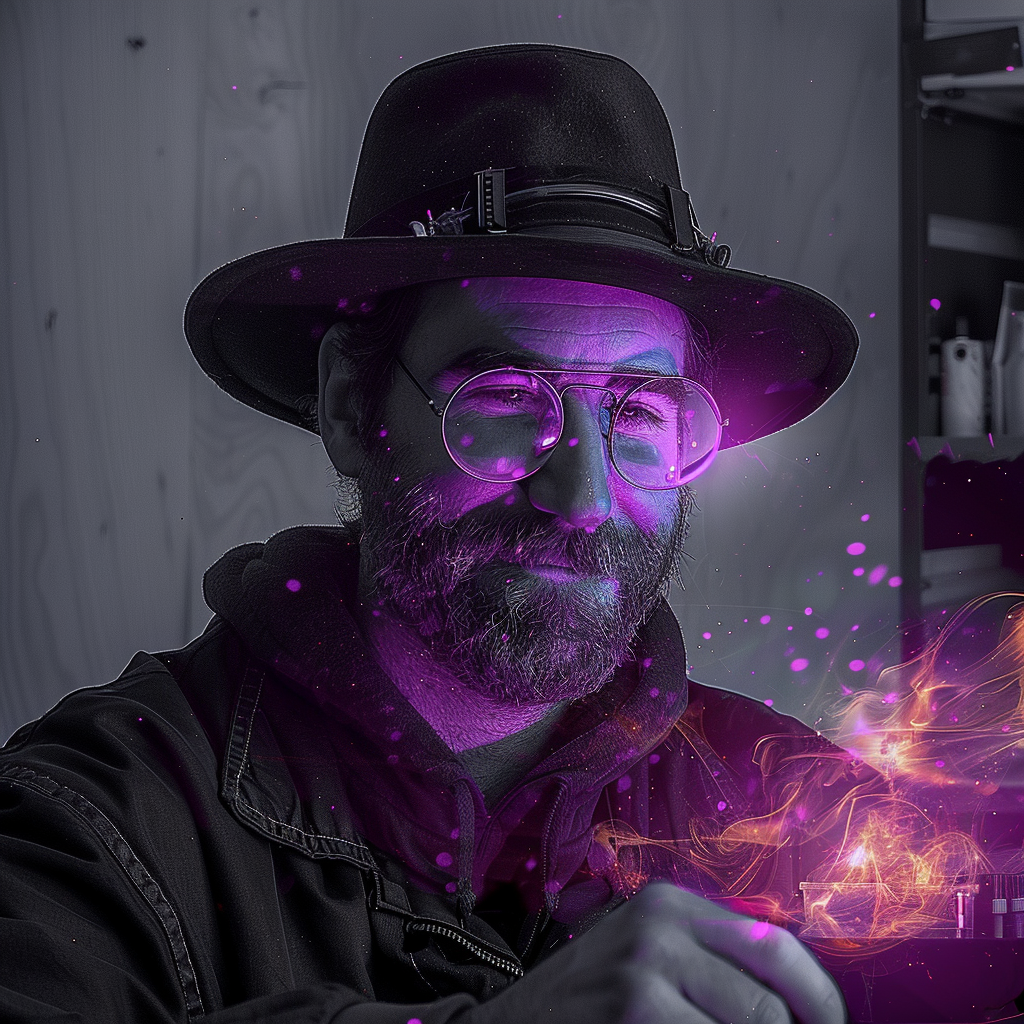
\includegraphics[width=3.8cm]{CHO.png}
      };
    \end{tikzpicture}

    \column{0.6\textwidth}
    \textbf{\Large Dr. John O'Hare}\\[0.3cm]
    \textcolor{elegantgray}{Chief Hallucination Officer, DREAMLAB}\\[0.5cm]

    \begin{itemize}
      \impactitem{primaryblue}{25+ years at tech's edge}
      \impactitem{successgreen}{VR pioneer → AI leader}
      \impactitem{warningorange}{PhD collaborative tech}
      \impactitem{modernpurple}{HP AI Lighthouse Partner}
    \end{itemize}

    \vspace{0.3cm}
    \textit{\small "This workshop distills decades of experience into skills you can use immediately."}
  \end{columns}
\end{frame}

% Why Choose Us - Differentiators
\ContentBackground
\begin{frame}[t]
  \frametitle{Why This Workshop Is Different}

  \begin{columns}[T]
    \column{0.33\textwidth}
    \centering
    \textcolor{primaryblue}{\Huge\faUsers}\\[0.3cm]
    \textbf{Small Cohorts}\\
    \small Max 10 participants\\Personal attention\\Peer learning

    \column{0.33\textwidth}
    \centering
    \textcolor{successgreen}{\Huge\faProjectDiagram}\\[0.3cm]
    \textbf{Real Projects}\\
    \small Work on YOUR tasks\\Immediate application\\Practical results

    \column{0.33\textwidth}
    \centering
    \textcolor{warningorange}{\Huge\faInfinity}\\[0.3cm]
    \textbf{Lifetime Access}\\
    \small Alumni community\\Quarterly workshops\\Ongoing support
  \end{columns}

  \vspace{0.8cm}
  \begin{modernblock}[Unique Advantages]{deepblue}
    \centering
    Vendor-agnostic • Privacy-first • Cross-industry insights • Future-proof skills
  \end{modernblock}
\end{frame}

% Next Steps - Call to Action
\ModernBackground{slide-17-backdrop.png}
\begin{frame}[t]
  \frametitle{Secure Your Transformation}

  \begin{modernblock}[Next Cohorts - Limited to 10 Seats]{primaryblue}
    \Large
    \begin{itemize}
      \item \textbf{March 2025:} 17-21 March \textcolor{warningorange}{(3 seats left)}
      \item \textbf{May 2025:} 12-16 May \textcolor{successgreen}{(Early bird open)}
      \item \textbf{July 2025:} 14-18 July (Just announced)
    \end{itemize}
  \end{modernblock}

  \vspace{0.5cm}

  \begin{columns}[T]
    \column{0.5\textwidth}
    \textbf{Simple Process:}
    \begin{enumerate}
      \item Online application (5 min)
      \item Screening call (15 min)
      \item £500 deposit
      \item Pre-course access
      \item Join cohort Discord
    \end{enumerate}

    \column{0.5\textwidth}
    \centering
    \vspace{0.5cm}
    \begin{tcolorbox}[colback=accentcyan!20,colframe=accentcyan,boxrule=3pt,arc=3mm]
      \centering
      \Large\textbf{workshops@dreamlab.uk}\\[0.3cm]
      \faPhone\quad +44 20 XXXX XXXX
    \end{tcolorbox}
  \end{columns}
\end{frame}

% Final Slide - Powerful Close
\ModernBackground{slide-18-backdrop.png}
\begin{frame}[plain]
  \begin{tikzpicture}[remember picture,overlay]
    % Dramatic gradient
    \shade[top color=deepblue,bottom color=primaryblue,opacity=0.95]
      (current page.south west) rectangle (current page.north east);
  \end{tikzpicture}

  \centering
  \vspace{3cm}
  {\color{white}\Huge\textbf{The Choice Is Clear}}\\[0.8cm]
  {\color{white!80}\Large Remain limited by consumer AI tools...}\\[0.5cm]
  {\color{white}\LARGE\textbf{OR}}\\[0.5cm]
  {\color{accentcyan}\Large\textbf{Master professional AI that transforms how you work}}\\[1.5cm]

  \begin{tcolorbox}[colback=white,colframe=white,boxrule=0pt,arc=3mm,width=0.6\textwidth]
    \centering
    \Large\textbf{workshops@dreamlab.uk}\\[0.3cm]
    \normalsize Join the 5\% who command AI with precision
  \end{tcolorbox}
\end{frame}

\end{document}